\subsection{Kociemba's Two Phase Algorithm}
This subsection will explain how the Kociemba Two Phase Algorithm works and why it can solve any \rubik{} in 29 \twist{}s or less. Kociemba's Algorithm finds a solution to a scrambled \rubik{} using to phases.

\subsubsection{Relabeling}
The relabeling process  starts with choosing an up face with a corresponding down face. Then choosing a front face with a corresponding back face. Each \facelet{} with the color of the up or down face is marked with the letters ``UD''. Each edge cube with a \facelet{} with the front or back face color and \textbf{not} the up or down face color on the other \facelet{} is marked with the letters ``FB''. Figure \ref{fig:relabel1} shows an example.

\begin{figure}[hb]
	\centering
		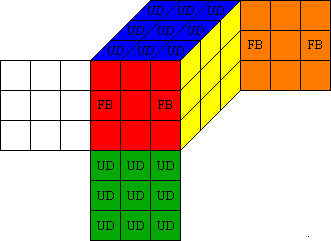
\includegraphics{input/pics/relabel1}
	\caption{\myCaption{A relabeled Rubik's Cube with the up and down faces blue and green respectively, and red and orange as front and back. The grayed facelets are relabeled.}}
	\label{fig:relabel1}
\end{figure}

When relabeling a \rubik{} in the position $s$ it is written as: $r(s)$. A \rubik{} in any position, $s$, is said to be en the set of positions called $H$ if and only if: $r(s)=r(e)$.

The following moves are in the set of moves $A$: U, U', U2, D, D', D2, R2, L2, F2 and B2. If using move sequences in $A$ on a position in $H$, the cube will always be in $H$.
